% 	HTML5 Robot User Interface Project Report: Introduction
% 	An ASLab Project,
% 	Developed by Daniel Peiró
% 	ETSII, UPM 2014-2015
\chapter{Introduction} \label{introduction}
The objective of this project is the development of software that provides a graphical user interface (hereinafter, GUI) 
with a variety of tools designed to gather inputs for the control of robots as well as the presentation of the output data 
from the robots themselves. The goal is that the application will comply with all of the following requirements:
\begin{itemize}
	\item \textbf{Universal}: The GUI must be easily adaptable for use in a wide array of robots, with different features 
	and lack thereof.
	\item \textbf{Accessible}: This is a two-fold requirement:
	\begin{itemize}
		\item The GUI must be easily usable from a wide array of devices, including but not limited to desktop and laptop 
		computers, mobile devices such as smartphones and tablets, all running different operating systems, which the 
		application should be agnostic of.
		\item The application that provides the GUI must also expose an API (Application Programming Interface) that enables 
		external developers to use the inputs and outputs from the GUI, so that the first requirement can be truly attained, 
		by adapting them to whatever application necessary. This interface should be as simple as possible, and comply with 
		all other requirements, where applicable (i.e. it must be portable, distributed, real-time capable and open source).
	\end{itemize}
	\item \textbf{Customizable}: Partially as a result of the first requirement, the GUI must have a variety of inputs and 
	outputs that can be used independently from one another, so that multiple configurations can be setup and used for 
	different robots, and different applications of the same robot. If possible, the user should be able to tailor custom 
	inputs and outputs when the proposed tools are insufficient for the particular application. This process should be 
	seamless and transparent for the user, when possible.
	\item \textbf{Distributed}: Partially as a result of the accessibility requirement, the application must be distributed 
	over a network, in such a way that the GUI need not be physically tethered to a particular machine, or locally executed 
	for the application to function.
	\item \textbf{Real-Time}: The inputs registered by the GUI must be able to control the robot in real-time, as well as 
	receive output from the robot in real-time. No hard real-time deadlines are set, given that the application is 
	distributed, these deadlines would be hard to estimate without extensive research and control over the environment of 
	the application, hence negating the accessibility requirement. However, the response time of the system should be 
	minimized to the extent of the current state of the art of the technologies used.
	\item \textbf{Portable}: The application that provides the GUI must be deployable on a wide array of systems with 
	regards to these variables:\\
		\begin{itemize}
			\item Hardware Capabilities: The application must be deployable on portable, affordable, low-end computers, as 
			to be easily mountable on mobile robots if so required.
			\item Operating System: The application must be multi-platform, meaning it can be deployed on a variety of 
			operating systems. These OSs must include at least, but not necessarily limited to: a general purpose Linux 
			distribution, Microsoft Windows and Apple OS X. Only the latest versions of each need to be supported. Required 
			Architectures, though not necessarily limited to: 32/64-bit x86.\\
		\end{itemize}
	\item \textbf{Open Source}: All of the software APIs, Libraries and Frameworks that are used in the application must be 
	open source. This generally entails that the software is free to use, study and modify, for any purpose. See section 
	\ref{opensourcemovement} of this report for more on open source software. The tools used for development (IDEs, OS, 
	Hardware etc.) need not be open source, but will be preferable if available.\\
\end{itemize}
In essence, what the application needs to do is bridge the two main entities of robot control:
\begin{itemize}
	\item \textbf{The User}: Needs an interface to input commands for the robot to follow. Also needs a view of the output data from the robot, if any is available.
	\item \textbf{The Robot}: Needs to receive commands in the particular protocol it understands, in order to function. Also, optionally, may output data for the user to consume or register.
\end{itemize}
The following simplified UML (Unified Modeling Language) diagram shows the three components: The user, the application, and the robot. The objective of this project is the development of the center component, the application, along with the interfaces it exposes both to the User and the Robot, or more accurately, the robot controller, which will translate the application's interface to the interface understood by the robot.
\begin{figure}[H]
\centering
\captionsetup{justification=centering}
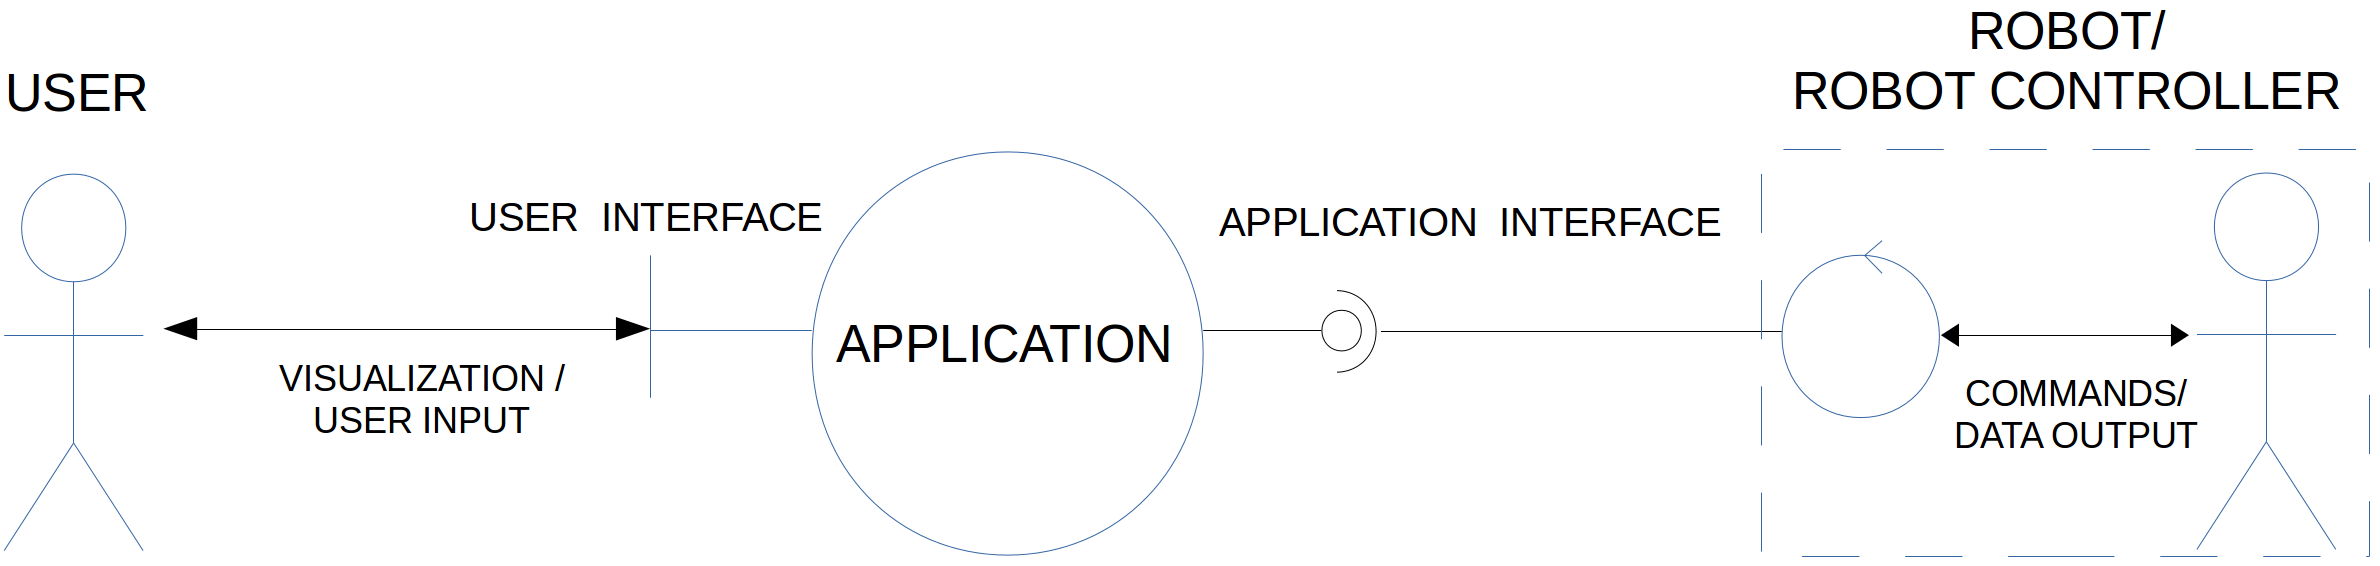
\includegraphics[width=\linewidth]{introuml}
\caption{Simplified UML Diagram of Project Objectives}
\end{figure}
\newpage
The current state of the art of the technologies that comply with these requirements and diagram were analyzed, a system 
architecture was designed, and the solution was developed and tested. These tasks are documented and discussed in chapters 
\textbf{\ref{technologyoverview}. Technology Overview} and \textbf{\ref{systemarchitecture}. System Architecture} 
respectively. The basic features and components of the solution are as follows. Of course, each of these is explained in 
detail in the previously cited chapters:
\begin{itemize}
	\item \textbf{HTML5 Modular Front-end}: The GUI is an HTML5 compliant web page. This proposes a solution for the first 
	accessibility requirement, since HTML5 web pages are accessible from any device capable of using a web browser. This 
	includes desktop and laptop computers, smartphones and tablets, as well as a variety of microcomputers. The modularity 
	gives a solution to the overall customization requirement, since every module can be executed independently from 
	another, any permutation of modules can be used.
	\item \textbf{Node.js Server Back-end}: The application is a Node.js web server. Given that Node.js is a multi-platform 
	framework, that runs on all the required architectures and operating systems listed and more, and is also very 
	lightweight, this proposes a solution to the portability requirement.
	\item \textbf{Client-Server Architecture}: This proposes a solution to the distributed requirement. The client is the 
	HTML5 web page that holds the GUI. The server is the application that manages inputs and outputs to and from the client. 
	Each can be executed on different machines, communicating over the Internet and local networks using a variety of 
	protocols.
	\item \textbf{WebSocket based communications}: This communication protocol allows the client and server to communicate 
	in real-time on a network, efficiently, by passing messages with associated data-packets, similarly to how processes 
	communicate through UNIX sockets. This proposes a solution for the real-time requirement.
	\item \textbf{MVC Architecture}: Proposes a solution for the universality and second accessibility requirements, by 
	designing the application so that the GUI (View) is decoupled from the state of the application (Model), allowing 
	external developers to design Controllers for any robot. This is called \textbf{double-decoupling} in this project.	
	\item \textbf{Custom Inputs and Outputs}: As a result of the first and the previous feature, it's possible for the user 
	to create new inputs and outputs on the fly, that are accessible to the API required by the second accessibility 
	requirement. This proposes a solution for the customization requirement.
	\item \textbf{Open Source}: All the technologies used are open source. A list of the external APIs and libraries used is 
	available on the second page of the references of this report.
\end{itemize}
The results of the proposed solution are exposed in chapter \textbf{\ref{conclusions}. Conclusions}.\\

This project is part of the ASLab (Autonomous System Laboratory) Robot Control Testbed (RCT) framework. This is a collection 
of mobile robot systems that are used to test the technologies developed in the Autonomous Systems Project (ASys). The main 
robot chosen for the RCT is a well known Pioneer 2AT8 robot nicknamed Higgs. With this robot the extent to which the 
developed autonomy software is capable of improving the performance of the robot in the execution of its missions is tested. 
In particular, the extent to which making Higgs self-aware will improve the robots resilience and robustness is tested (Sanz 
et al., 2007; Hernández, 2013). The focus of this project is the construction of a new user interface that complies with all 
the previously stated requirements, for the visualization and control of the robot state. There are two previous 
implementations:
\begin{itemize}
	\item Based on the extant user interfaces provided by the ROS (Robot Operating System) middleware and it's associated 
	stacks. This requires the ROS middleware for execution (hence limiting the portability of the UI).
	\item The Android Robot Interface (ARI)- that runs on an Android device (Mata, 2013).
\end{itemize}
This project enables the remote use of the Higgs robot (or any other robot) from any browser able to handle HTML5.